\subsection{Theoretical Basis}
\label{subsec:theoretical-basis}

The project focuses on web crawling and PageRank computation to analyze the structure and importance of web pages within a specific domain.
Web crawling systematically browses the internet to collect hyperlinks, forming a directed graph where nodes represent web pages and edges represent hyperlinks.
The crawling process ensures that only valid URLs within the target domain are collected, excluding static files like images or PDFs to maintain relevance.

PageRank, developed by Google, is an algorithm that assigns importance scores to web pages based on their link structure.
It models the behavior of a random surfer who navigates the web by following links with probability $d$ (damping factor, typically 0.85) or jumps to a random page with probability $1-d$.
The PageRank score for a page $p_i$ is computed iteratively using the formula:
\begin{equation}
    PR(p_i) = \frac{1-d}{N} + d \sum_{p_j \in M(p_i)} \frac{PR(p_j)}{L(p_j)}
    \label{eq:page_rank}
\end{equation}
where $N$ is the total number of pages, $M(p_i)$ is the set of pages linking to $p_i$, $L(p_j)$ is the number of outgoing links from page $p_j$, and $d$ is the damping factor.
This iterative process converges when the difference between successive rank estimates falls below a tolerance threshold.

\subsection{Implementation}
\label{subsec:implementation}

The implementation consists of three main components: a web crawler to collect URL pairs, a PySpark-based framework for data processing, and a PageRank algorithm to compute page importance.
The system is designed to handle large-scale data efficiently, leveraging parallel processing and distributed computing.

\subsubsection{Crawler Function - Adjacency Matrix Initialization}\text{}

The web crawler is implemented in Python using the \texttt{requests} and \texttt{BeautifulSoup} libraries to fetch and parse web pages.
The \texttt{crawl\_website} function starts from a seed URL (\texttt{https://it.tdtu.edu.vn}) and collects unique (source, destination) URL pairs, representing directed edges in the web graph.
It ensures that only URLs within the target domain are included and excludes static files (e.g., .jpg, .pdf) using the \texttt{is\_valid\_url} function.
The crawler uses a set to store unique edges, avoiding duplicates, and saves the results to a CSV file (\texttt{url\_pairs.csv}). The crawler initializes the adjacency matrix implicitly by collecting edges, which are later processed to form the graph structure for PageRank computation.

\subsubsection{PySpark Initialization}\text{}

To handle large-scale data, the project uses PySpark, a distributed computing framework, to process the crawled URL pairs and compute PageRank scores.
A Spark session is initialized to manage data as DataFrames, enabling scalable operations.
The edge data from the CSV file is loaded into a Spark DataFrame with columns \texttt{source} and \texttt{destination}.
The Spark configuration includes a checkpoint directory to manage intermediate results and prevent stack overflow during iterative computations.
The edges are loaded and processed to create a list of unique pages (nodes) and compute out-degrees for each source page, forming the basis for the PageRank algorithm.

\subsubsection{PageRank Implementation}\text{}

The PageRank algorithm is implemented in a \texttt{PageRank} class that takes the edge DataFrame, damping factor (0.85), maximum iterations (10), and tolerance (1e-4) as parameters.
The algorithm initializes ranks uniformly ($\frac{1}{N}$) for all pages and iteratively updates them based on contributions from incoming links.
It uses Spark's DataFrame operations for joins, aggregations, and broadcasting to optimize performance.
Checkpoints are used every three iterations to manage memory.
The algorithm outputs a DataFrame with page URLs and their corresponding PageRank scores, which are used for further analysis and visualization.

\subsection{Result Analysis}
\label{subsec:result-analysis}

The crawler collected 75,970 unique URL pairs from the \texttt{it.tdtu.edu.vn} domain, forming a directed graph of web pages.
The PageRank algorithm was applied to this graph, and the top 20 pages by rank were visualized using a directed graph, with node sizes proportional to their ranks.
The visualization was generated using the \texttt{networkx} and \texttt{matplotlib} libraries and saved as \texttt{top\_pages\_graph.png}.

\begin{figure}[H]
    \centering
    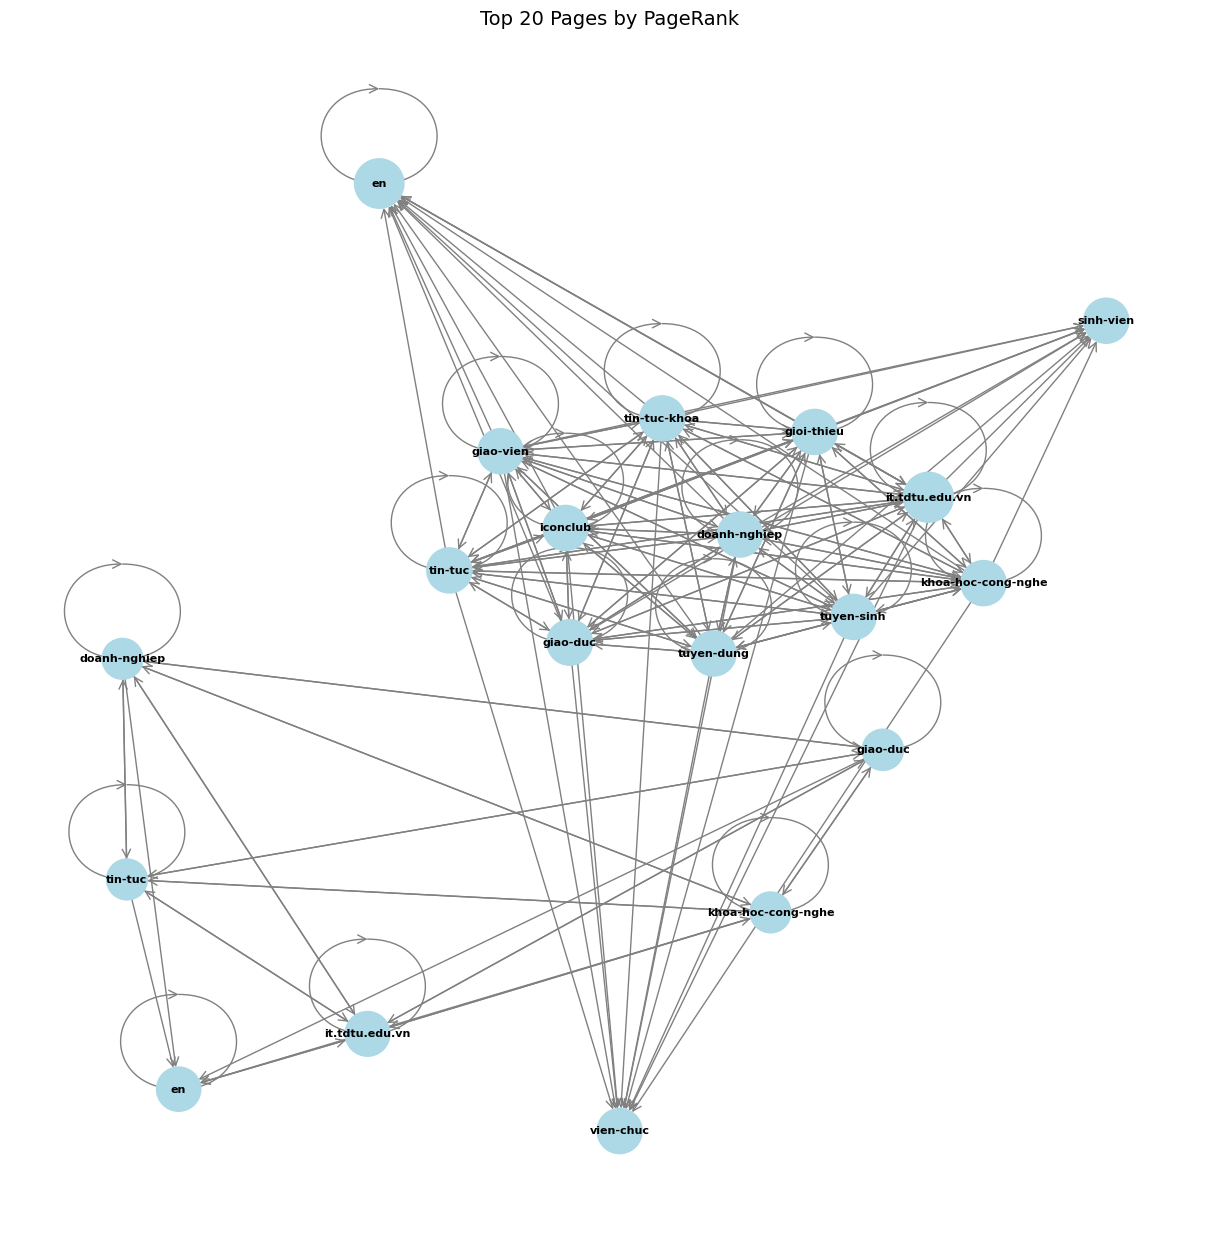
\includegraphics[width=0.6\linewidth]{images/top_pages_web}
    \caption{Directed graph of the top 20 pages by PageRank score, with node sizes proportional to ranks.}
    \label{fig:top_pages_graph}
\end{figure}

The most important page, with a PageRank score of approximately 0.01293, was \texttt{https://it.tdtu.edu.vn/}, the faculty homepage.
This high rank is expected, as the homepage is a central hub with many incoming links from other pages within the domain.
Other high-ranking pages included department-specific pages and key sections like \texttt{https://it.tdtu.edu.vn/en}, reflecting the students' most focused topics and subjects.